\[
	\Delta u = 0 \quad u \in W
\]
\[
	u|_s = f
\]

\[
	W = \frac{1}{r_{AP}}
\]
где $
	r_{AP} = \sqrt{(x - x_0)^2 + (y - y_0)^2 + (z - z_0)^2}
$
-- расстояние между точками $A(x, y, z)$ и $P (x_0, y_0, z_0)$.
\begin{align*}
	 &\derp{W}{x}{} = - \frac{1}{r_{AP}^2} \derp{r_{AP}}{x}{} = - \frac{1}{r_{AP}^2} \frac{2 (x - x_0)}{2 \sqrt{(x - x_0)^2 + (y - y_0)^2 + (z - z_0)^2}} = \frac{(x - x_0)}{r_{AP}^3}\\[10pt]
	&\derp{W}{x}{2} = - \frac{1}{r_{AP}^3} + \frac{3 (x - x_0)^2}{r_{AP}^5}; \quad \derp{W}{y}{2} = - \frac{1}{r_{AP}^3} + \frac{3 (y - y_0)^2}{r_{AP}^5}; \quad \derp{W}{z}{2} = - \frac{1}{r_{AP}^3} + \frac{3 (z - z_0)^2}{r_{AP}^5}; 
\end{align*}
\[
	\Delta u = - \frac{3}{r_{AP}^3} + \frac{3 [(x - x_0)^2 + (y - y_0)^2 + (z - z_0)^2]}{r_{AP}^5} = 0
\]
		Данное решение имеет в точке $A$ особенность.\\
\[
	\iint\limits_{S} \left(u \derp{v}{n}{} - v \derp{u}{n}{}\right) dS = \iint\limits_S \left(u \der{v}{n}{} - v \der{u}{n}{}\right) dS = \iiint\limits_{W} \left(u \Delta v - v \Delta u \right) d \omega
\]
		Решение $W = \frac{1}{r_{AP}}$ верно только в области $\omega$. Попробуем построить решение $W_1$ для всей области $W$.\\
		
		Построим функцию Грина\\
\[
	\Delta W_1 = 0 \quad W_1 |_S = W |_S
\]
\[
	G (x, y, z, x_0, y_0, z_0) = W_1 - W; \quad G|_S = 0
\]
		Предположим, что в функции Грина $v = G$. Тогда 
\[
	\iint\limits_{S} \left(u \derp{v}{n}{} - v \derp{u}{n}{}\right) dS = \iint\limits_S \left(u \der{v}{n}{} - v \der{u}{n}{}\right) dS = \iiint\limits_{W} \left(u \Delta v - v \Delta u \right) d \omega
\] %подписать что равно нулю
\[
	\iint\limits_{S} \left(u \derp{G}{n}{} \right) dS + \iint\limits_{S_1} \left(u \der{G}{n_1}{} - v \der{u}{n_1}{}\right) dS_1 = 0 
\]
		Перейдём к сферической системе координат.\\
\begin{figure}[h!]
	\centering
	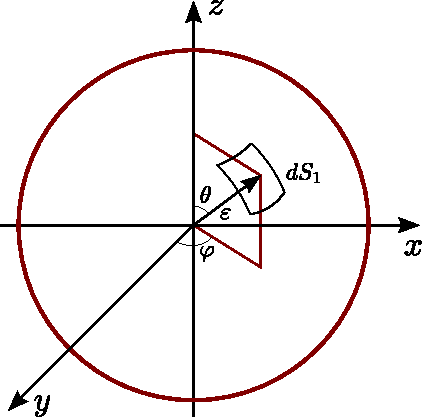
\includegraphics{figGreenIllust.pdf}
\end{figure}
\[
	dS_1 = \varepsilon^2 \sin \theta \, dv d \varphi
\]
\[
	\iint\limits_{S_1} \left(u \der{G}{n_1}{} - v \der{u}{n_1}{}\right) dS_1 = \int\limits_0^{2 \pi} d\varphi \int\limits_0^{\pi} \left(- u \der{G}{r}{} + G \der{u}{r}{} \right) \varepsilon \sin \theta d \theta
\]

\begin{multline*}
	\lim\limits_{\varepsilon \to 0} \iint\limits_{S_1} \left( u \derp{G}{u_1}{} - G \derp{u}{u_1}{} \right) ds = - \int\limits_{0}^{2 \pi} d \varphi \int\limits_{0}^{\pi} d\theta \sin \theta u = \\ = u (x_0, y_0, z_0)\int\limits_0^{2 \pi} d \varphi \int\limits_{0}^{\pi} \sin \theta d \theta = - 4 \pi u (x_0, y_0, z_0) 
\end{multline*}
\[
	u(x_0, y_0, z_0) = \frac{1}{4 \pi} \iint\limits_S f \derp{G}{u}{} dS
\]
Получили решение задачи Дирихле через функцию Грина.\\
Функцию Грина можно построить для шара, сферы и полупространства.\\